\documentclass[class=article, crop=false]{standalone}
\usepackage{tikz}
\usepackage{subcaption}
\usetikzlibrary{calc}
\usetikzlibrary {shapes.geometric}

\begin{document}
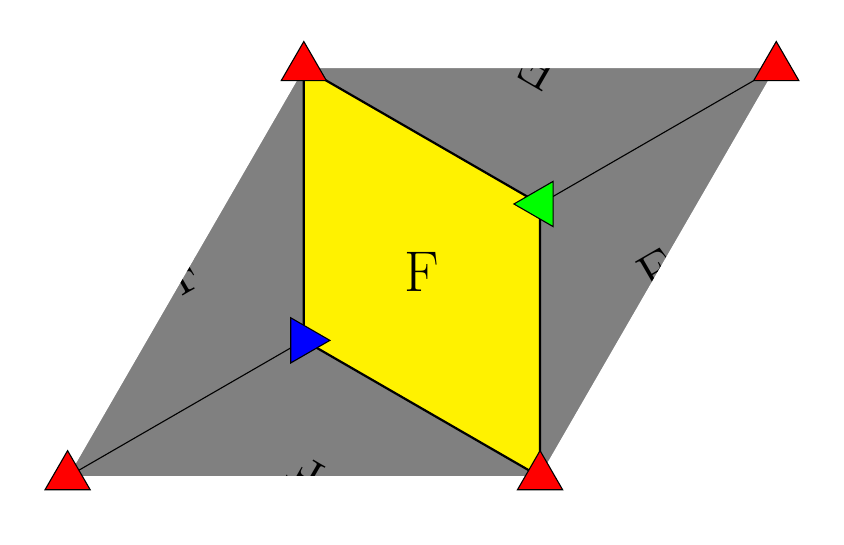
\begin{tikzpicture}
            % Define the lengths of the sides and the angle
            \def\a{3}  % length of side a
            \def\b{3}  % length of side b
            \def\angle{60}  % angle between sides a and b
            \def\s{F} % Label in center of cells

            \def\x{0.5} % Boundary 
            \def\y{0.5} % Boundary

        
            % Calculate the coordinates of the points
            \coordinate (C00) at (0, 0);
            \coordinate (C10) at (\a, 0);
            \coordinate (C11) at ({\a + \b*cos(\angle)}, {\b * sin(\angle)});
            \coordinate (C01) at ({\b * cos(\angle)}, {\b * sin(\angle)});
            \coordinate (C02) at ({2*\b*cos(\angle)}, {2*\b * sin(\angle)});
            \coordinate (C12) at ({\a +2*\b * cos(\angle)}, {2*\b * sin(\angle)});
            \coordinate (C22) at ({2*\a + 2*\b * cos(\angle)}, {2*\b * sin(\angle)});
            \coordinate (C21) at ({2*\a + \b*cos(\angle)}, {\b * sin(\angle)});
            \coordinate (C20) at ({2*\a}, 0);
        
            % Draw the oblique unit cell
            \draw[fill=gray,gray] (C00) -- (C20) -- (C22) -- (C02) -- cycle;
            \draw[thick,fill=yellow] ($(C00)!0.6666!(C11)$) -- (C20) -- ($(C11)!0.3333!(C22)$) -- (C02) -- cycle;

            
            % Draw boundary chiral centres
            \node[rotate=150] at (C10) {\huge \s};
            \node[rotate=30] at (C21) {\huge \s};
            \node[rotate=150] at (C12) {\huge \s};
            \node[rotate=30] at (C01) {\huge \s};

            % Create white border
            \draw[fill=white,white] ($(C00)-(\x,\y)$) -- ($(C20)-(-\x,\y)$) -- (C20) -- (C00);
            \draw[fill=white,white] ($(C00)-(\x,-\y)$) -- ($(C02)-(\x,-\y)$) -- (C02) -- (C00);
            \draw[fill=white,white] ($(C02)+(\x,\y)$) -- ($(C22)-(\x,-\y)$) -- (C22) -- (C02);
            \draw[fill=white,white] ($(C20)+(\x,-\y)$) -- ($(C22)+(\x,\y)$) -- (C22) -- (C20);

            % Draw chiral inner centre
            \node at (C11) {\huge \s};


            % Draw mirrow lines
            \draw (C00) -- ($(C00)!0.6666!(C11)$);
            \draw ($(C11)!0.3333!(C22)$) -- (C22);


            % Draw node reflections
            \draw (C00)  node[regular polygon, regular polygon sides=3, draw, fill=red, minimum size=0.5cm] {};
            \draw (C02)  node[regular polygon, regular polygon sides=3, draw, fill=red, minimum size=0.5cm] {};
            \draw (C22)  node[regular polygon, regular polygon sides=3, draw, fill=red, minimum size=0.5cm] {};
            \draw (C20)  node[regular polygon, regular polygon sides=3, draw, fill=red, minimum size=0.5cm] {};

            \draw ($(C00)!0.6666!(C11)$)  node[rotate = 30,regular polygon, regular polygon sides=3, draw, fill=blue, minimum size=0.5cm] {};
            \draw ($(C11)!0.3333!(C22)$)  node[rotate=90, regular polygon, regular polygon sides=3, draw, fill=green, minimum size=0.5cm] {};    
        \end{tikzpicture}
\end{document}